\documentclass{epflposter}
\usepackage{amssymb,amsmath}
\usepackage[default]{SuisseIntl}
\usepackage{graphicx}
\usepackage{physics}
\usepackage{setspace}
\usepackage{tikz}
\usepackage{pgfplots}
\pgfplotsset{width=13cm,compat=1.9}

\title{\parbox{50cm}{Non-Explosion for RDEs with Coefficients Having Unbounded Derivatives}}
\author{Xue-Mei Li and \underline{Kexing Ying}}
\institute{EPFL, Institute of Mathematics. Email: \underline{\texttt{kexing.ying@epfl.ch}}}


\begin{document}
\maketitle
\setstretch{1.1}

\begin{columns}
\column{0.5}
\block{Introduction}{
  Fix \(\mathbf{X} = (X, \mathbb{X})\) a rough path of \(\alpha \in (\frac{1}{3}, 1]\) regularity 
  (including Young regime) and \(b, \sigma\) (not necessarily bounded) vector fields, we consider the 
  RDE
  \[\dd Y_t = b(Y_t) \dd t + \sigma(Y_t) \dd \mathbf{X}_t.\]
  \textbf{Question:} What sufficient conditions on \(b, \sigma\) ensure that the RDE does not explode?
}

\block{Additive Noise: Spinning Out of Control}{
  For \(\sigma = 0\), we require \(b\) to have linear growth along the process
  (Osgood's criterion), i.e. 
  \begin{equation}\label{eq:linear_growth}
    \left\langle \frac{x}{\|x\|}, b(x)\right\rangle \le f(\|x\|) \text{ for some } 
    f \text{ s.t. } \int_{0+}^\infty \frac{1}{f(r)} \dd r = \infty.\tag{\(*\)}
  \end{equation}

  This turns out to be insufficient even for the case of additive noise, i.e. \(\sigma\) is some constant matrix.
  Consider of the 2-dimensional SDE 
  \[\dd x_t = \|x_t\|^5
    \begin{pmatrix}
      0 & -1\\
      1 & 0
    \end{pmatrix}x_t\ \dd t + \dd W_t.\]

    Easy to check for any initial condition, the SDE does not explode a.s.
  
  \vspace{5mm}
  Evolution of unit ball under same realization of the noise: 

  \begin{center}
    \begin{minipage}{0.9\linewidth}
      \centering
      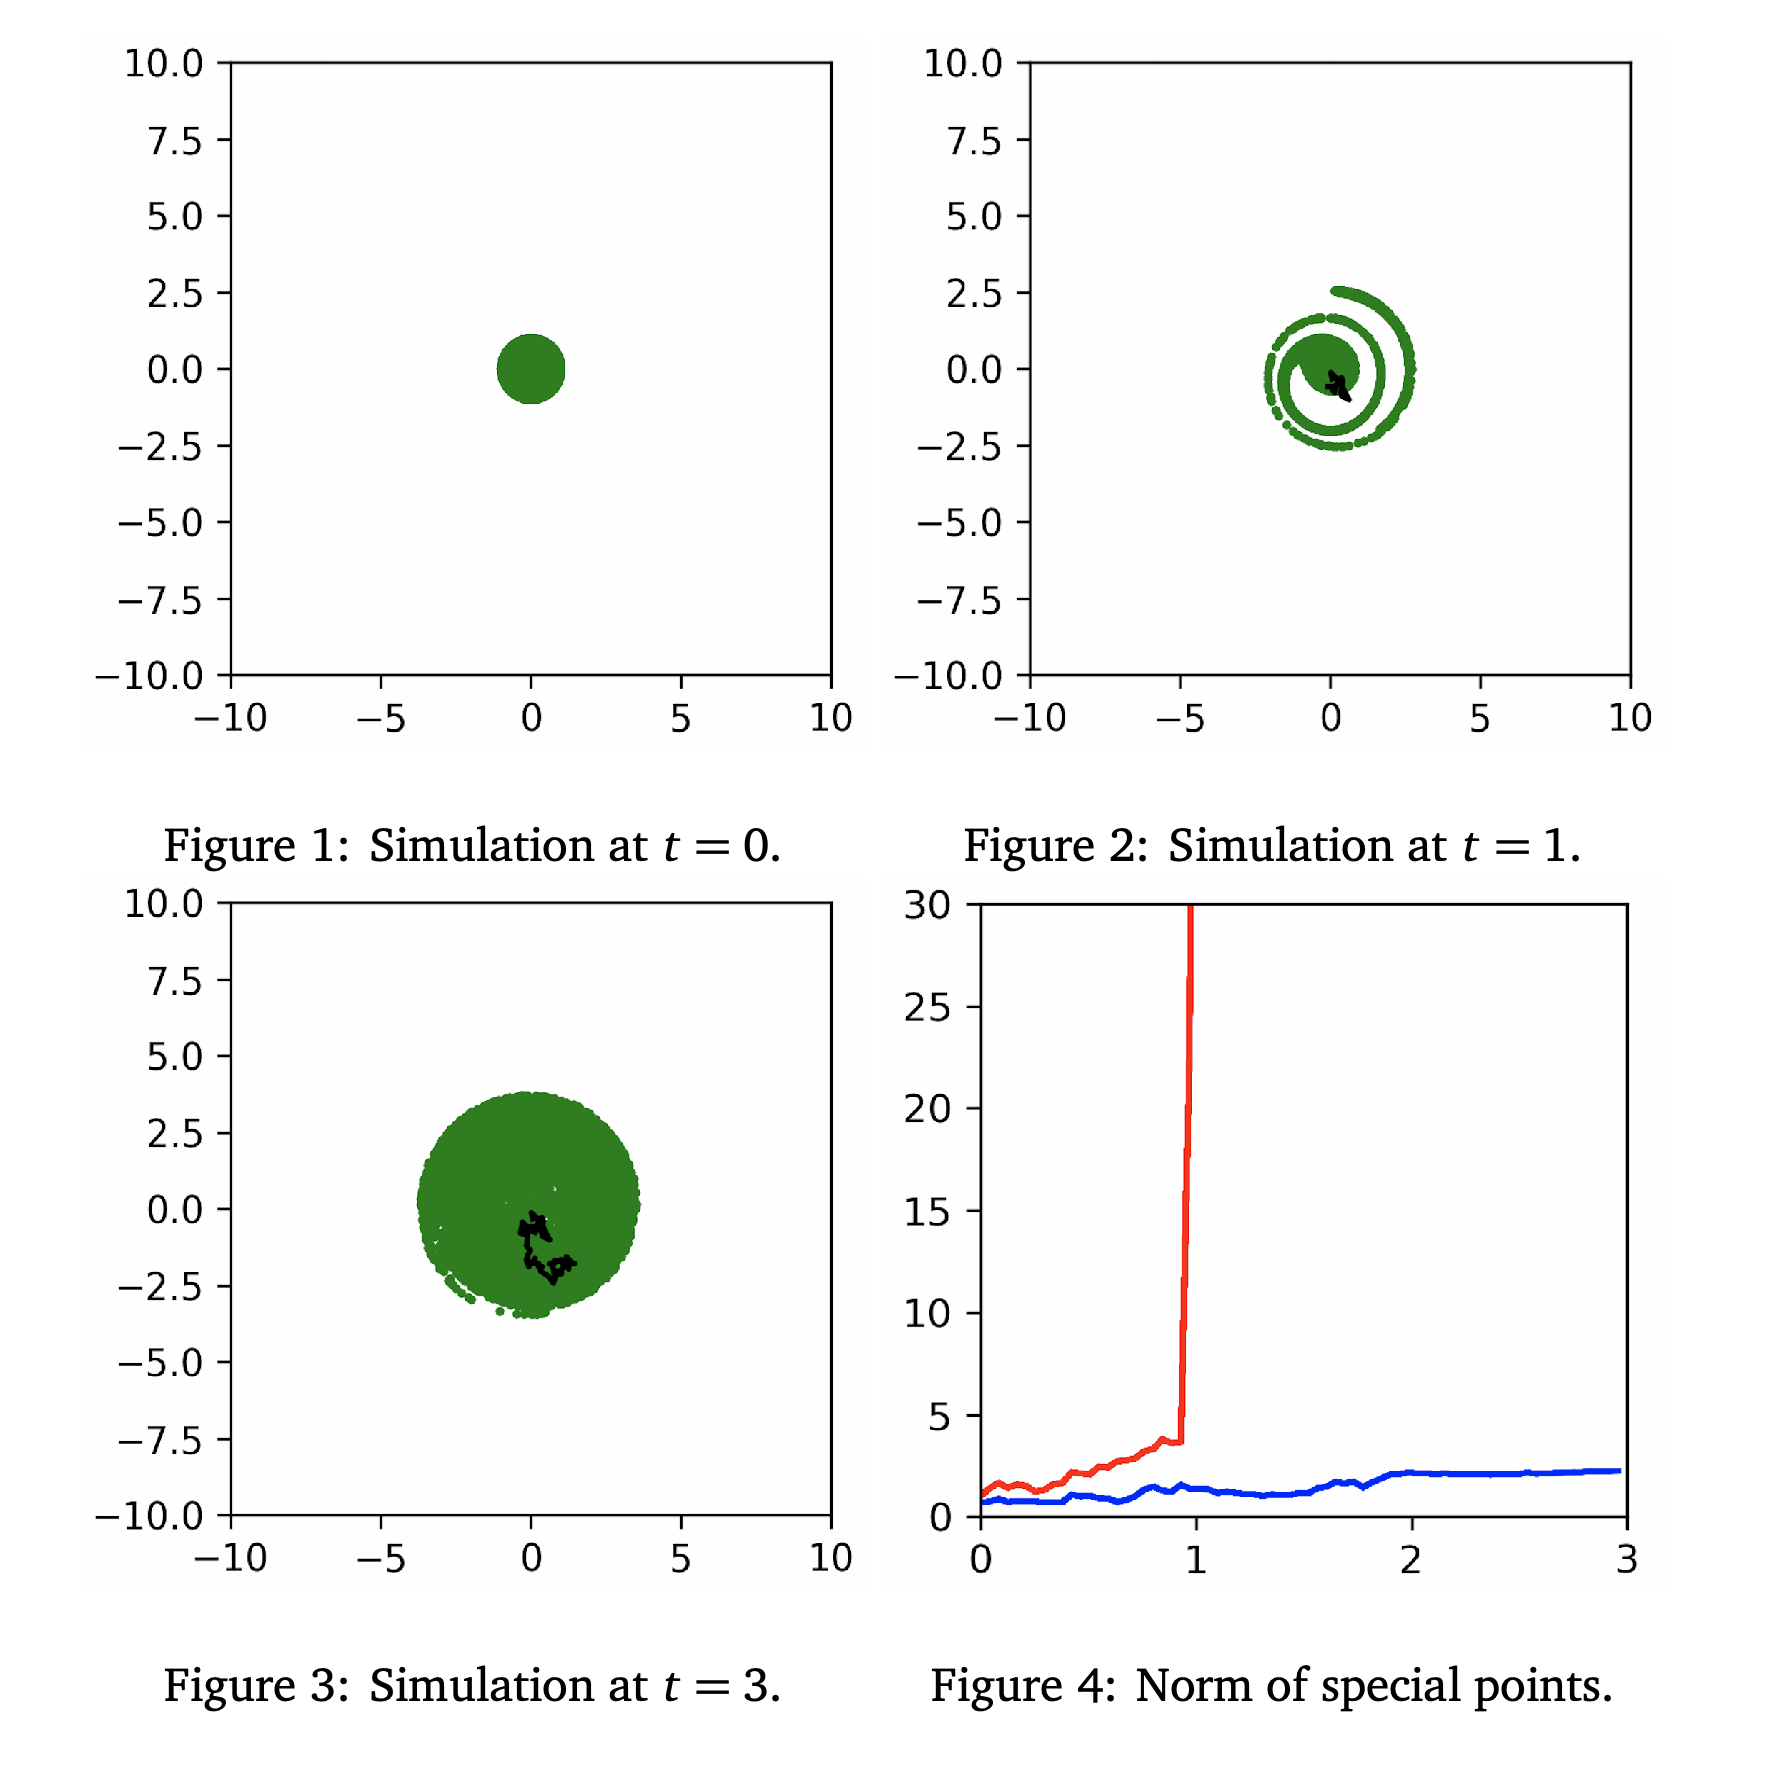
\includegraphics[width=\linewidth]{sim/sq.png}
    \end{minipage}
  \end{center}

  Denoting \(\phi\) for the flow of this SDE, the {\color{red} Red line} is 
  \(\sup_{\|x\| \le 1} \|\phi_t(x)\|\) and the {\color{blue} Blue line} is 
  \(\frac{1}{\pi}\int_{\|x\| \le 1}\|\phi_t(x)\| \dd x\).
  Namely, for fixed realization, the SDE explodes for some initial condition!
  Thus, taking \(\mathbf{X}\) the It\^o lift of a Brownian motion provides a counter-example.

  \vspace{5mm}
  \textit{Explicit} and \textit{deterministic} construction of a counter-example also exists (c.f. Section 3.3 of \cite{Li:25}). 
}

\block{Additive Noise: Criterion}{
  For ODE with additive noise \(\dd x_t = b(x_t) \dd t + \dd \xi_t\), we provide the following 
  sufficient and \textit{sharp} criterion for non-explosion
  \begin{itemize}
    \item \(\xi \in C^\alpha\) for some \(\alpha \in (0, 1)\) (\(\alpha = 1\) can be dealt directly);
    \item Equation~\eqref{eq:linear_growth} holds and moreover, for all \(x \perp y\)
    \[\left|\left\langle \frac{y}{\|y\|}, b(x)\right\rangle\right| \le (1 + \|x\|)f(\|x\|)^\beta\]
    for some \(\beta \le 1 + \alpha\).
  \end{itemize}
  Namely, more regular noise \(\implies\) more growth of \(b\) allowed.
  
  \vspace{1.5mm}
  Similar result hold replacing H\"older regularity by \(p\)-variation.
}

\column{0.5}
\block{Rough Differential Equations}{ 
  For \(b = 0\), consider the RDE
  \[\dd \begin{pmatrix}Y_t^1\\Y^2_t\end{pmatrix} 
    = \begin{pmatrix}Y_t^1 \sin Y_t^2\\ Y_t^1\end{pmatrix} \dd \mathbf{X}_t\]
  with \(\mathbf{X}_t = (0, t \otimes t)\) explodes \(\implies\) linear growth condition is insufficient.

  Moreover, for \(\mathbf{X}\) the It\^o lift of a Brownian motion, \(\sigma\) bounded and smooth 
  is insufficient for non-explosion (c.f. \cite{Li:11}).

  \vspace{5mm}
  Simple criterion when \(b = 0\) \cite[Theorem 3.12]{Gubinelli:25}: 
  RDE does not explode if \(\|D\sigma\|_\infty, \|D^2\sigma\|_\infty < \infty\). 

  \vspace{5mm}
  \innerblock{Unbounded derivatives}{
    We provide a sufficient condition for non-explosion when \(b \neq 0\) and \(\sigma\) has 
    unbounded derivatives (stated here for \(\alpha \in (\frac{1}{3}, \frac{1}{2}]\)):
    \begin{itemize}
      \item \(b\) satisfies Equation~\eqref{eq:linear_growth} and \(\|b(x)\| \le f(\|x\|)^{1 + \kappa \alpha}\);
      \item and \(\|D^n \sigma(x)\| \le f(\|x\|)^{(1 - n\kappa)\alpha -}\) for \(n = 0, 1, 2\)
    \end{itemize}
    for some \(\kappa \in [0, \frac{1}{2})\).
  }

  \innerblock{Decaying second derivatives (WIP)}{
    If \(\sigma\) has decaying second derivative, we can achieve a non-explosion criterion with 
    better growth condition while still 
    allowing unbounded first order derivative (here we take \(b = 0\) and \(\alpha \in (\frac{1}{3}, \frac{1}{2}]\)):
    \begin{itemize}
      \item \(\|D\sigma(x)\| \lesssim (\log (1 + \|x\|))^{\alpha}\);
      \item \(\|D^n\sigma(x)\| \lesssim (1 + \|x\|)^{(1 - n)\gamma}\) for \(n = 0, 2\).
    \end{itemize}
    for some \(\gamma \in [\alpha, 2\alpha)\).
  }

  \innerblock{Going further downwards (WIP)}{
    For \(\alpha < \frac{1}{3}\), same argument holds interpreting the integral as a branched 
    rough integral. This allows arbitrarily close to linear growth of by dropping down a level of regularity, 
    e.g. treating a \(\frac{2}{5}\)-H\"older rough path as a \(\frac{1}{3}-\epsilon\) branched rough path via 
    its canonical lift.
  }
}

\begingroup
\colorlet{framecolor}{epflred}
\block{Proof Sketch}{
  Treating the rough integral \(\eta_t := \int_0^t Y_s \dd \mathbf{X}_s\) as the noise part of an ODE 
  with additive noise, we can apply the previous criterion if we can estimate its regularity on a 
  partition of the time interval. 

  For \(\alpha \in (\frac{1}{2}, 1]\), apply sewing lemma to obtain the desired estimate.

  For \(\alpha \in (\frac{1}{3}, \frac{1}{2}]\), estimate from sewing lemma gives a non-linear 
  inequality and na\"ive estimate no longer works.

  \textbf{Key lemma:} \textit{uniform} estimate for class of functions \(f\) satisfying a (non-linear) inequality 
  \[a(f(\epsilon)) \le \epsilon b(f(\epsilon)) \text{ for all } \epsilon > 0.\]
  
  \textit{Idea:} Cannot live in any region other than the first one as all others vanish in the limit \(\epsilon \to 0\).
  \begin{center}
    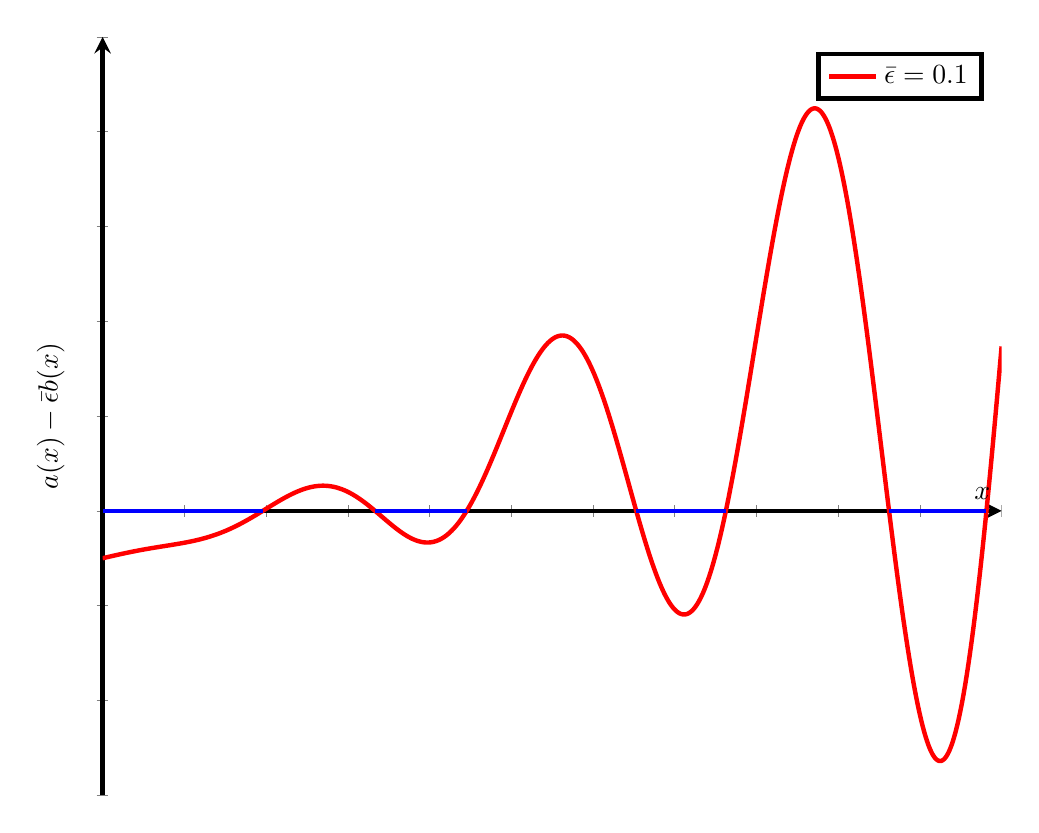
\begin{tikzpicture}
      \begin{axis}[
          legend style={fill=white,draw=black},
          axis x line = middle,
          axis y line = left,
          xmin=0,
          xmax=22, 
          ymin=-30,
          ymax=50,
          xlabel = $x$,
          ylabel = {$a(x)- {\bar \epsilon} b(x)$},
          xticklabel=\empty,
          yticklabel=\empty,
          style={ultra thick},
      ]
      \addplot [
          domain=0:22, 
          samples=1000, 
          color=red,
      ]
      {x - 5 - (x^2 * sin(deg(x)) / 10)};
      \addlegendentry{${\bar\epsilon} = 0.1$}
      \addplot [
          domain=0:3.9204, 
          samples=2, 
          color=blue,
          style={ultra thick},
      ]
      {0};
      \addplot [
          domain=6.66771:8.9098, 
          samples=2, 
          color=blue,
          style={ultra thick},
      ]
      {0};
      \addplot [
          domain=13.05858:15.25156, 
          samples=2, 
          color=blue,
          style={ultra thick},
      ]
      {0};
      \addplot [
          domain=19.24436:21.62772, 
          samples=2, 
          color=blue,
          style={ultra thick},
      ]
      {0};
    \end{axis}
    \end{tikzpicture}
    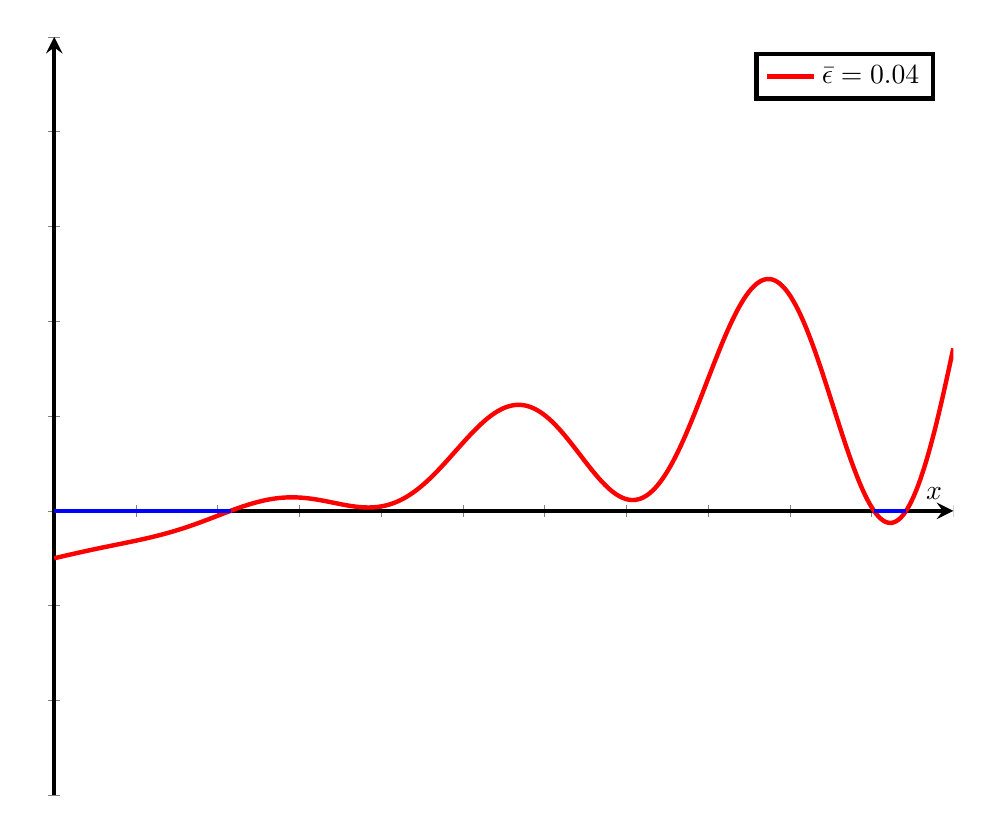
\begin{tikzpicture}
      \begin{axis}[
          legend style={fill=white,draw=black},
          axis x line = middle,
          axis y line = left,
          xlabel = $x$,
          xmin=0,
          xmax=22, 
          ymin=-30,
          ymax=50,
          xticklabel=\empty,
          yticklabel=\empty,
          style={ultra thick},
      ]
      \addplot [
          domain=0:22, 
          samples=1000, 
          color=red,
      ]
      {x - 5 - 0.04 * (x^2 * sin(deg(x)))};
      \addlegendentry{${\bar\epsilon} = 0.04$}
      \addplot [
          domain=0:4.31392, 
          samples=2, 
          color=blue,
          style={ultra thick},
      ]
      {0};
      \addplot [
          domain=20.05962:20.84378, 
          samples=2, 
          color=blue,
          style={ultra thick},
      ]
      {0};
    \end{axis}
    \end{tikzpicture}
  \end{center}
  In our case \(\epsilon\) is the interval size and \(f\) is the H\"older norm.
}
\endgroup

\block{\Large References}{
  \small
  \begingroup
  \renewcommand{\refname}{}     
  \setlength{\parskip}{0pt}        
  \vspace{-3.5em}                   
  \bibliographystyle{alpha}
  \bibliography{refs}
  \endgroup
}

\end{columns}


\end{document}

